\renewcommand*{\arraystretch}{1.1}

\subsection*{Interactive / short / 3}
\label{section:interactive-short-read-03}



\noindent\begin{tabularx}{\queryCardWidth}{|>{\queryPropertyCell}p{\queryPropertyCellWidth}|X|}
	\hline
	query & Interactive / short / 3 \\ \hline
%
	title & Person Friends
 \\ \hline
%
	pattern & \hfill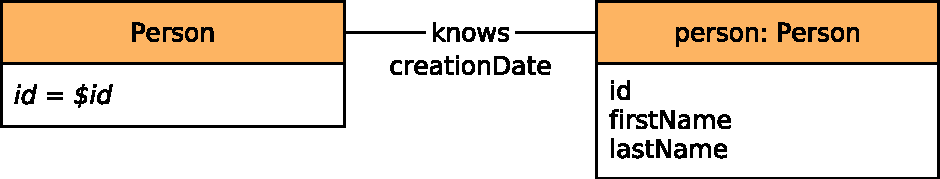
\includegraphics[scale=\patternscale,margin=0cm .2cm]{patterns/interactive-short-read-03}\hfill\vadjust{} \\ \hline
%
	desc. & Given a start Person, retrieve all of their friends, and the date at
which they became friends.
 \\ \hline
%
	
		params &
		\innerCardVSpace{\begin{tabularx}{\attributeCardWidth}{|>{\paramNumberCell}c|>{\varNameCell}M|>{\typeCell}m{\typeWidth}|Y|} \hline
		$\mathsf{1}$ & Person.id
 & ID
 &  \\ \hline
		\end{tabularx}}\innerCardVSpace \\ \hline
	
%
	
		result &
		\innerCardVSpace{\begin{tabularx}{\attributeCardWidth}{|>{\resultNumberCell}c|>{\varNameCell}M|>{\typeCell}m{\typeWidth}|>{\resultOriginCell}c|Y|} \hline
		$\mathsf{1}$ & Person.id & ID & R &
				 \\ \hline
		$\mathsf{2}$ & Person.firstName & String & R &
				 \\ \hline
		$\mathsf{3}$ & Person.lastName & String & R &
				 \\ \hline
		$\mathsf{4}$ & Knows.creationDate & DateTime & R &
				 \\ \hline
		\end{tabularx}}\innerCardVSpace \\ \hline
	
%
	
		sort		&
		\innerCardVSpace{\begin{tabularx}{\attributeCardWidth}{|>{\sortNumberCell}c|>{\varNameCell}M|>{\directionCell}c|Y|} \hline
		$\mathsf{1}$ & Knows.creationDate
 & $\desc
$ &  \\ \hline
		$\mathsf{2}$ & Person.id
 & $\asc
$ &  \\ \hline
		\end{tabularx}}\innerCardVSpace \\ \hline
	%
	%
	%
	%
\end{tabularx}
\queryCardVSpace